\documentclass[titlepage]{article}
\usepackage{setspace}
\doublespacing
\usepackage{siunitx}
\usepackage[version=4]{mhchem}
% \documentclass{memoir}
% \usepackage{chemfig}
% \renewcommand*\printatom[1]{\ensuremath{\mathsf{#1}}}

% Language setting
% Replace `english' with e.g. `spanish' to change the document language
\usepackage[english]{babel}

% Set page size and margins
% Replace `letterpaper' with `a4paper' for UK/EU standard size
\usepackage[letterpaper,top=2cm,bottom=2cm,left=3cm,right=3cm,marginparwidth=1.75cm]{geometry}

% Useful packages
\usepackage{amsmath}
\usepackage{graphicx}
\graphicspath{ {./images} }
\usepackage[colorlinks=false, allcolors=blue]{hyperref}

\title{\Huge{Chemistry Honors \\ MX Lab Analysis}}
\author{\huge{Oh, Justin} \and \huge{Ye, Nathan}}
\date{\LARGE{\today}}


\begin{document}
\maketitle

% \tableofcontents

\begin{abstract}

In this lab, we are given two mystery elements labeled M and X and tasked to figure out the identity of the two through various tests. Different elements have unique properties that can tell us the identity of them. We can exploit these different properties through various tests that can clearly show the identity of some mystery element. Through this lab, we hope to gain and practice the knowledge we have learned. We will also be able to practice our lab skills and understanding of safety. Being able to tell similar-looking materials apart is also crucial, one wrong chemical used will ruin an experiment in the best case and expose people to deadly chemicals. Before we started running tests, we hypothesized that M is zinc and X is iodine though visual inspection and logical deduction. We factored in cost, safety, and compatibility just to name a few. By use of visual inspection and a conductivity test, we were able to determine that M was a metal. There were many methods we used to determine the identity of M: flame test, reactivity test, melting point. To determine the identity of X, we used visual inspection. Our results showed that M had a blueish white flame, a in the middle reactivity, and a very similar melting point to zinc. When heated up X started releasing purple vapors. From our testing, we can confidently state that M is zinc and X is iodine and our two guesses were both correct. 

%\chemfig{I-Zn-I}

% \chemfig{C*6(-C(-[32/6]H)(-[40/6]H)-C(-[40/6]H)(-[0]H)-C(-[0]H)(-[8/6]H)-C(-[8/6]H)(-[16/6]H)-C(-[16/6]H)(-[4]H)-)(-[4]H)(-[32/6]H)}

\end{abstract}

%! add a table of contents
\tableofcontents
\newpage

\section{Background}
We initially observe that \textbf{M} is made of small pieces cut from a sheet and appears to be metallic. We also see that it has a not particularly shiny, but untarnished appearance. By considering these visual properties, as well as the safety and price of materials, we narrow our initial guesses down to aluminium and zinc, two relatively common, safe metals that come in sheets. Between these two guesses, we choose \emph{zinc} as our first guess for \textbf{M}, as the appearance of \textbf{M} is very similar to zinc samples that we have encountered in previous labs.
\begin{figure}[h]
    \centering
    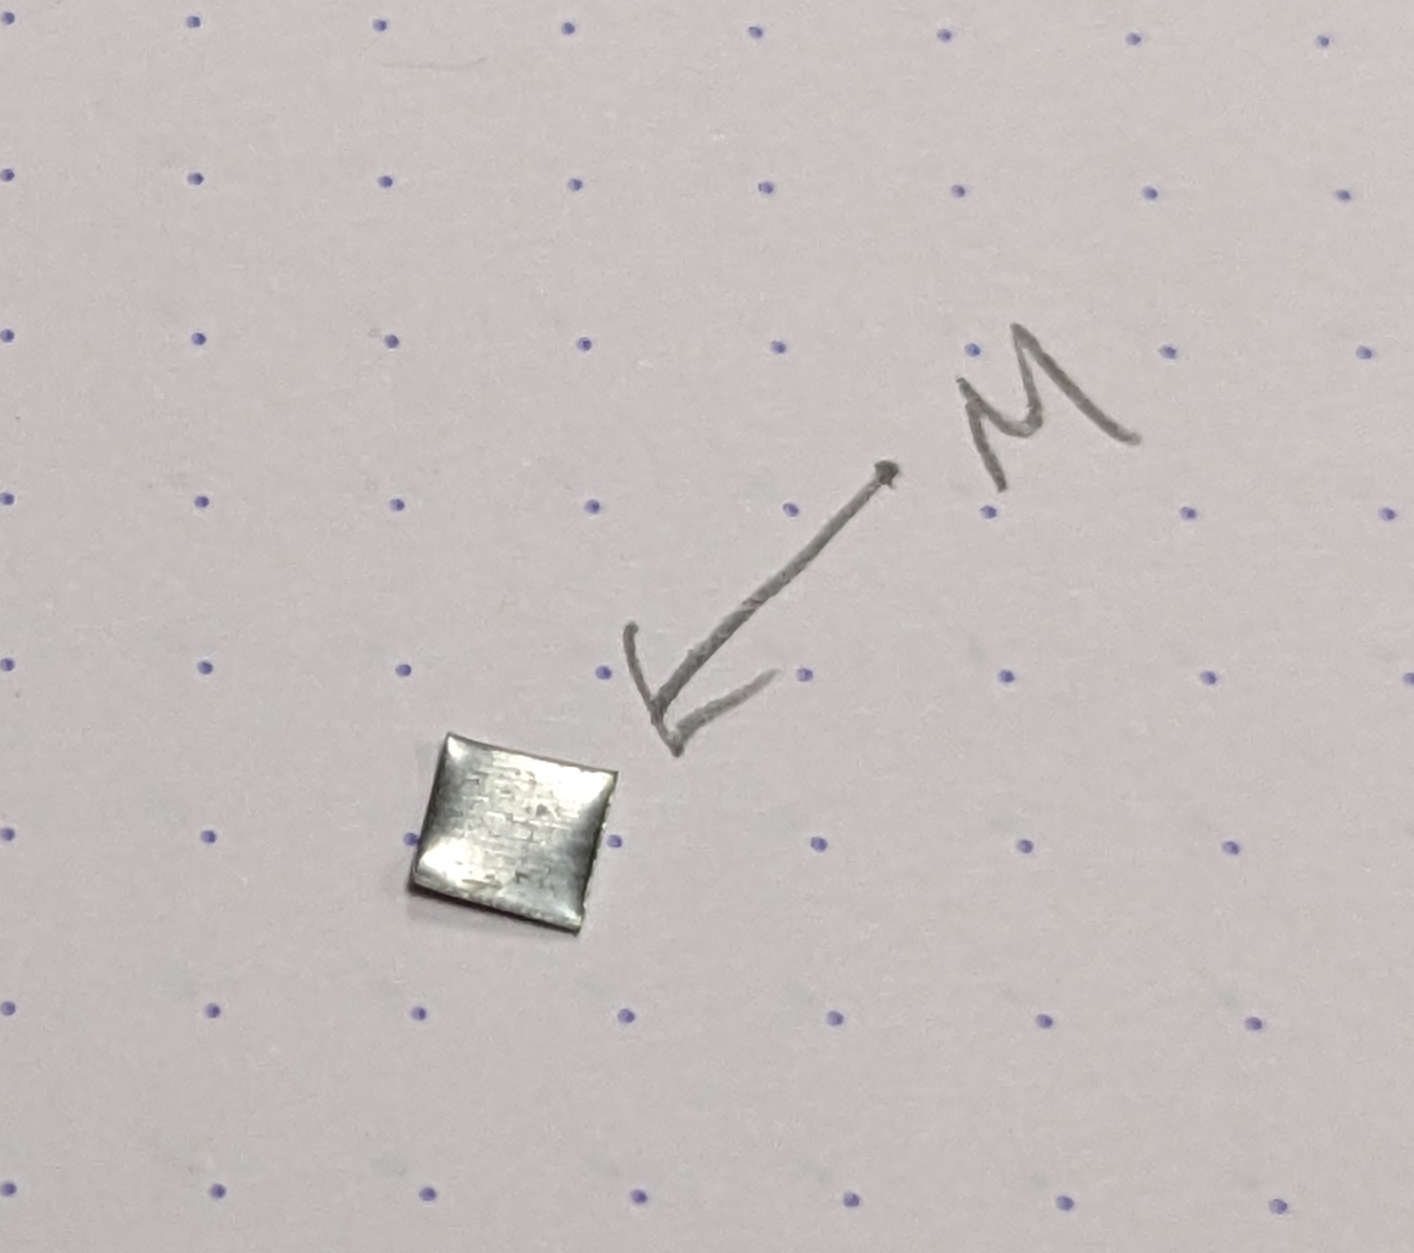
\includegraphics[height=3cm]{unknown_M.jpg}
    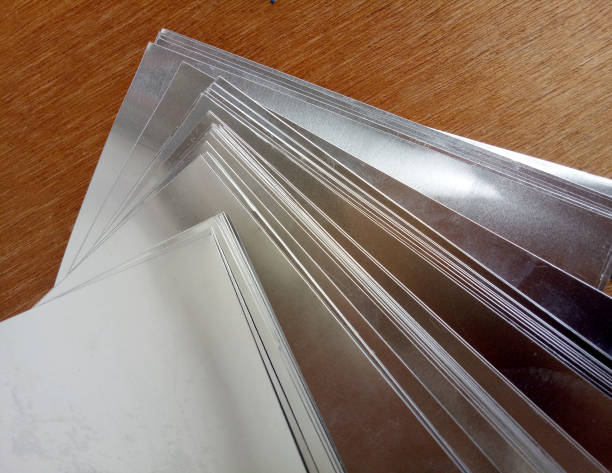
\includegraphics[height=3cm]{aluminium_sheet.jpg}
    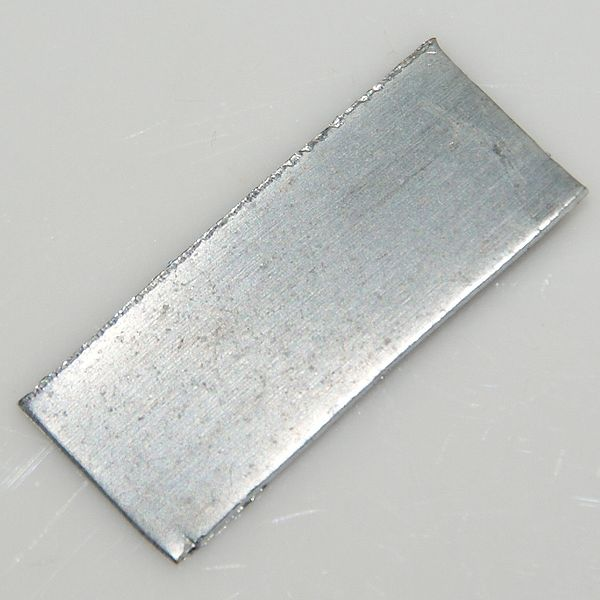
\includegraphics[height=3cm]{zinc_sheet.jpg}
    \caption{From left to right: \textbf{M}, aluminium sheets, zinc sheet}
    \label{fig:m_comparison}
\end{figure}

As for \textbf{X}, we observe that it is made of dark, nearly black, pieces that are fairly crystalline. Using its color, we came up with an initial pool of guesses for \textbf{X}: beryllium, boron, carbon, phosphorous, arsenic, selenium, or iodine. Due to safety factors, we chose to eliminate beryllium, phosphorus, arsenic, and selenium from our initial guesses, as they pose a serious safety risk to humans. Having considered basic appearance and safety, we are left with boron, carbon, and iodine as initial guesses. We choose to test for \emph{iodine} first, as boron and carbon are both inert at room temperature, and would be significantly harder to react with \textbf{M}.
\begin{figure}[h]
    \centering
    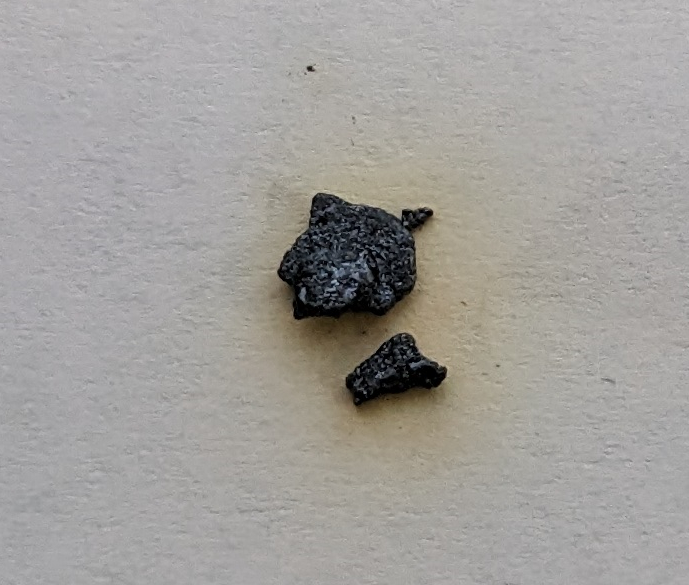
\includegraphics[height=3cm]{unknown_X.jpg}
    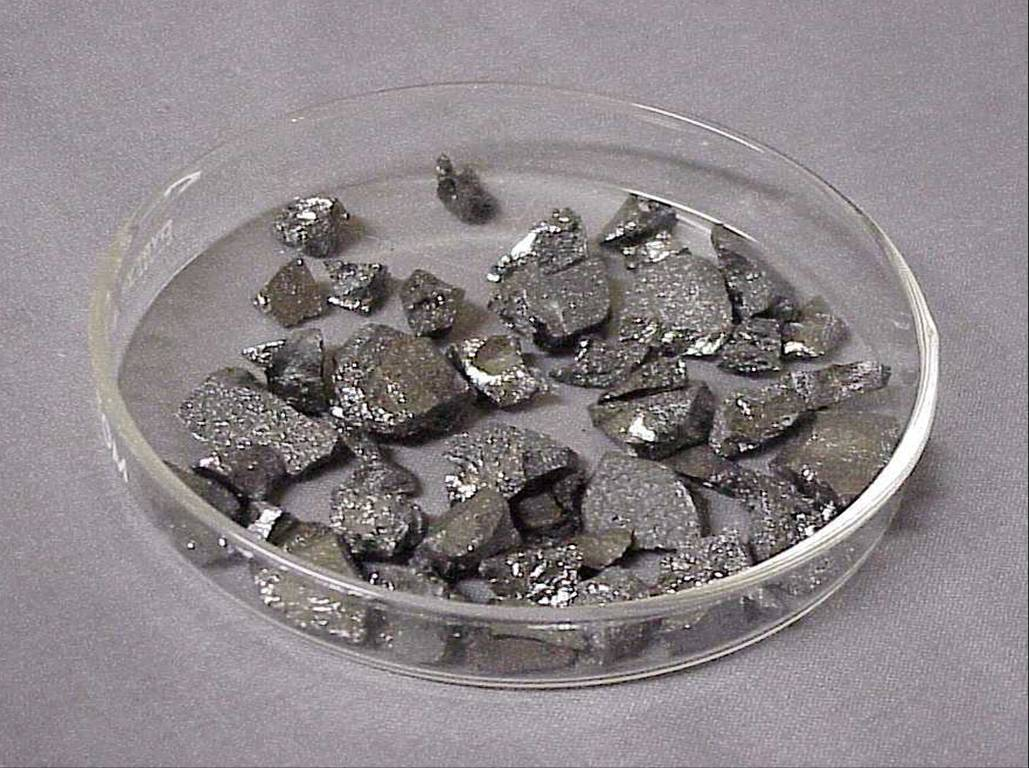
\includegraphics[height=3cm]{boron.jpg}
    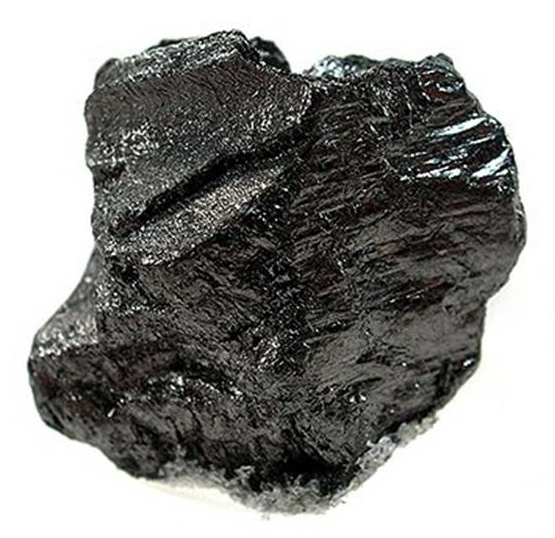
\includegraphics[height=3cm]{graphite.jpg}
    \includegraphics[height=3cm]{iodine.jpg}
    \caption{From left to right: \textbf{X}, boron, graphite, iodine}
    \label{fig:x_comparison}
\end{figure}

If our initial guesses of \emph{zinc} and \emph{iodine} are correct, we would expect a reaction between them to produce \emph{zinc iodide}. 
\begin{displaymath}
    \ce{Zn + I2 -> ZnI2}
\end{displaymath}
Since zinc iodide is an ionic salt that is soluble in water, we would expect our product to be aqueous if synthesized in water or some other solvent, otherwise, we would expect a solid product. Since zinc iodide is an ionic compound, we would expect it to have certain properties that are intrinsic to ionic compounds, such as a very high melting point and conductivity when dissolved in water. These properties will be very useful in confirming its synthesis. If our product is synthesized in solution, we can recover the solid form by evaporating off the solvent.
\bigskip

Using dimensional analysis and the balanced chemical equation for our reaction, we can see that for every gram of iodine consumed, we will need 0.25790 grams of zinc. This ratio lets us know that for an equal mass of zinc and iodine, iodine will be the limiting reagent in the reaction, as less zinc is consumed per unit mass of iodine. Therefore, in a reaction with an equal mass of zinc and iodine, we would expect to find excess zinc remaining after the reaction.
\begin{gather*}
    \ce{Zn + I2 -> ZnI2} \\[2ex]
    \SI{1}{\gram\of{I}}\times\frac{\SI{1}{\mol\of{I}}}{\SI{126.90}{\gram\of{I}}}\times\frac{\SI{1}{\mol\of{Zn}}}{\SI{2}{\mol\of{I}}}\times\frac{\SI{65.380}{\gram\of{Zn}}}{\SI{1}{\mol\of{Zn}}}=\SI{0.25760}{\gram\of{Zn}}
\end{gather*}

% maybe combine 3 paragraphs into 1
% i think ill number the sections off like section for just X and M and then subsection them into the indiv tests
We initially planned to measure the density of the materials as a quick way to determine if our guesses were close, however, we found that the masses of unknowns given to us were too small to be able to accurately determine density with the precision of our instruments. To verify the identity of \textbf{M}, we can first confirm that \textbf{M} is a metal beyond visual observation by testing its malleability and conductivity. Once we have verified that \textbf{M} is indeed a metal, we have two major options in order to verify its identity. 

The first of these is the activity series. By attempting to react our unknown with various aqueous ionic solutions, we can determine if \textbf{M} is more or less reactive than the cation in the solution. By testing against a variety of ionic compounds, we can determine where on the activity series \textbf{M} lies, which will allow us to identify it. 

The second test we can perform is a flame test. By exciting \textbf{M} ions by means of a flame, the ion will emit light as a product of its electrons rising and falling between energy levels. By observing the color of this flame, we can determine the identity of \textbf{M}.
\bigskip

We can first perform more general tests on \textbf{X} in order to eliminate groups of elements. For example, we can test for lack of conductivity to verify that \textbf{X} is not a metal. In order to confirm our hypothesis of iodine as \textbf{X}'s identity, we can search for distinctive properties of iodine in \textbf{X}. Perhaps iodine's most distinctive characteristic is the visible purple gas that it sublimes\footnote{Following the definition where solid transitions directly to gas, not necessarily occurring below the triple point} into when heated in its solid form at room temperature. If \textbf{X} sublimes into a purple gas, we will be very certain that it is indeed iodine.
% don tyou just not need to footnote after the 1st reference (which is on the page above)

\section{Materials}
% center these
\begin{tabular}{ |c|c| } 
 \hline
 \multicolumn{2}{| c |}{Chemicals} \\
 \hline
 Name & Concentration \\
 \hline
 \ce{AgNO3(aq)} & \SI{0.1}{\mol\per\liter} \\ 
 \ce{AgNO3(aq)} & \SI{0.1}{\mol\per\liter} \\ 
 \ce{AgNO3(aq)} & \SI{0.1}{\mol\per\liter} \\ 
 \ce{AgNO3(aq)} & \SI{0.1}{\mol\per\liter} \\ 
 \ce{HNO3(aq)} & \SI{0.1}{\mole\per\liter} \\ 
 \ce{CH3OH} & \SI{1234}{\percent} \\
 cell7 & cell8 \\ 
 \hline
\end{tabular}
\quad
\begin{tabular}{ |c|c| } 
 \hline
 \multicolumn{2}{| c |}{Glassware} \\
 \hline
 Name & Concentration \\
 \hline
 \ce{AgNO3(aq)} & \SI{1}{\mol\per\liter} \\ 
 \ce{HNO3(aq)} & \SI{0.1}{\mole\per\liter} \\ 
 \ce{CH3OH} & \SI{1234}{\percent} \\
 cell7 & cell8 \\ 
 \hline
\end{tabular}
\quad
\begin{tabular}{ |c|c| } 
 \hline
 \multicolumn{2}{| c |}{Other Equipment} \\
 \hline
 Name & Concentration \\
 \hline
 \ce{AgNO3(aq)} & \SI{1}{\mol\per\liter} \\ 
 \ce{HNO3(aq)} & \SI{0.1}{\mole\per\liter} \\ 
 \ce{CH3OH} & \SI{1234}{\percent} \\
 cell7 & cell8 \\ 
 \hline
\end{tabular}

\section{Procedures}

Our first step was to visually observe \textbf{M} and \textbf{X} and hypothesized based on characteristics such as color and uniformity. Just based on this we were able to form our hypothesis of what the two elements could be.

\begin{figure}[h]
    \centering
    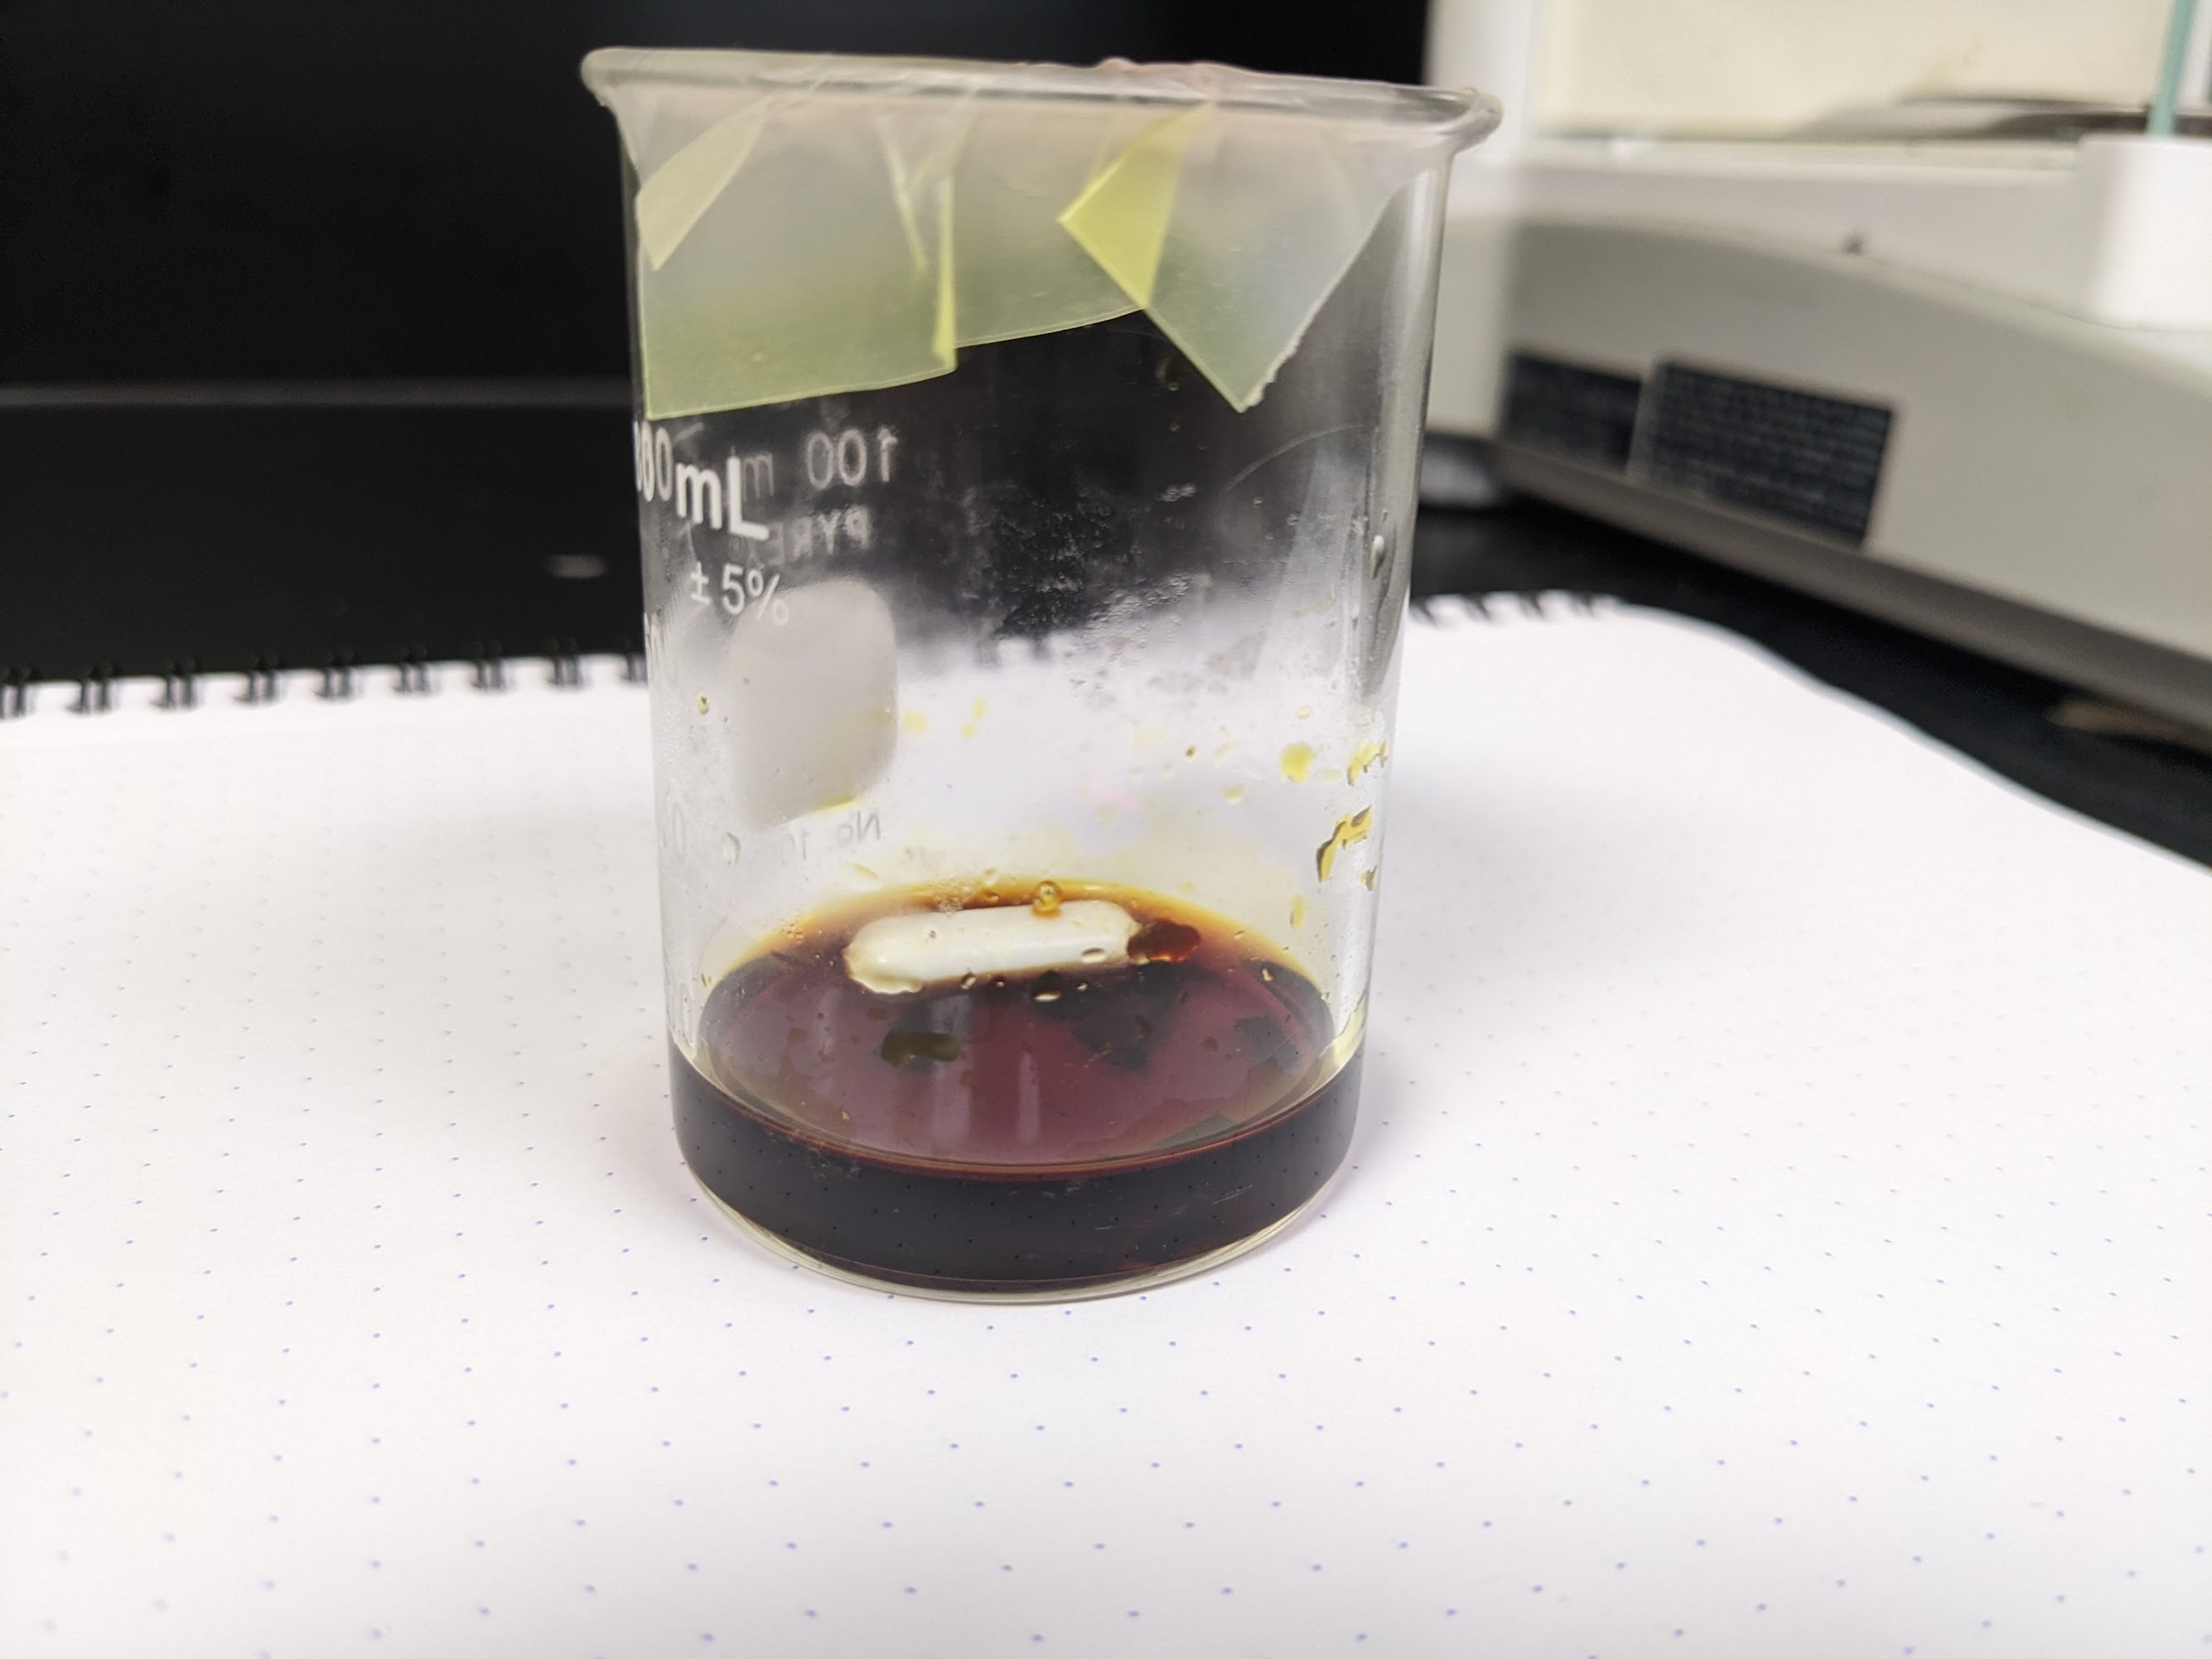
\includegraphics[height=3cm]{MX_initial.png}
    % you switched them :skull:
    % the lighter one is final
    % oops ur right shhhhhhhhhh :skull: my brain is dead
    %ITS NOT WORKINGGNNGNGNGG
    % ill just crop then upload
    % no point in trying to crop it in latesx
    % alright
    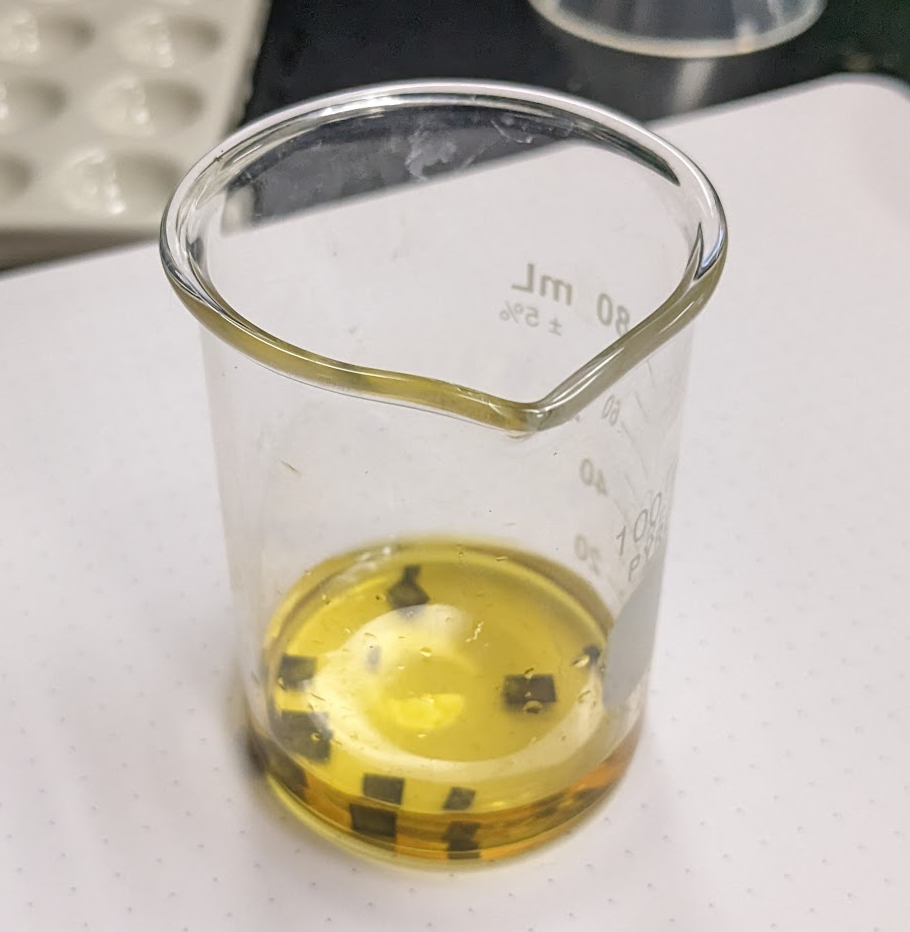
\includegraphics[height=3cm]{MX_final.png}
    \caption{On the left: \ce{M + X} combined initially, on the right: \ce{M + X} after two days}
    \label{fig:mx_comparison}
\end{figure}

In the directed portion of this lab, we weighed an equal amount of \textbf{M} and \textbf{X} and recorded how much we used: 0.512$\pm$0.001\unit{\gram\of{\textbf{M}}} and 0.494$\pm$0.001\unit{\gram\of{\textbf{X}}}. We then measured 8.60\unit{\milli\liter} of 'water' using a 10\unit{\milli\liter} graduated cylinder and poured it into a 100\unit{\milli\liter} beaker. \textbf{M} and \textbf{X} were then added to the beaker. We added a stir bar, covered the beaker with parafilm, and placed the beaker on the stir plate. We ran the stir plate over the course of the period, uncovered the beaker to remove the stir bar, covered it back up and let it sit over two days as we waited for a reaction to occur. Throughout this process, we recorded our observations. When \textbf{X} was added to the 'water' it quickly became a dark purplish shade, and after sitting for two days, the mixture had turned much lighter and had a yellow tint (Fig. \ref{fig:mx_comparison}). We then needed to filter off the liquid to get rid of impurities and unreacted solids then evaporate off the liquid. We set up a ring stand with a funnel that led to an evaporation dish. In the funnel a folded coffee filter was put. We then poured the contents of the beaker into the funnel and waited for it to finish draining. Once finished we set the evaporation dish aside and cleaned up the filtration setup. To speed up the evaporation process, we put the evaporation dish on the hot plate and turned it to a very low setting. Once all the liquid was gone and it started smoking a bit, we immediately took the dish off the hot plate and waited for it to cool down. We measured the mass of the dish with product to be 55.380$\pm$0.001\unit{\gram} and the dish by itself to be 55.903$\pm$0.001\unit{\gram}. This gives us a yield of 0.523$\pm$0.001\unit{\gram\of{\textbf{{MX}}}}. We also observed this product to be a white powder.

\begin{figure}[h]
    \centering
    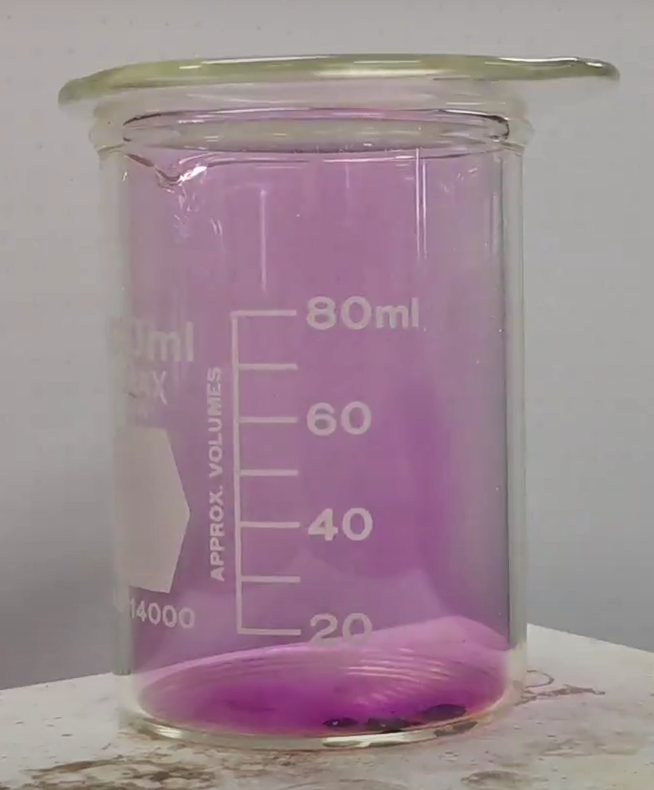
\includegraphics[height=3cm]{iodine_gas.png}
    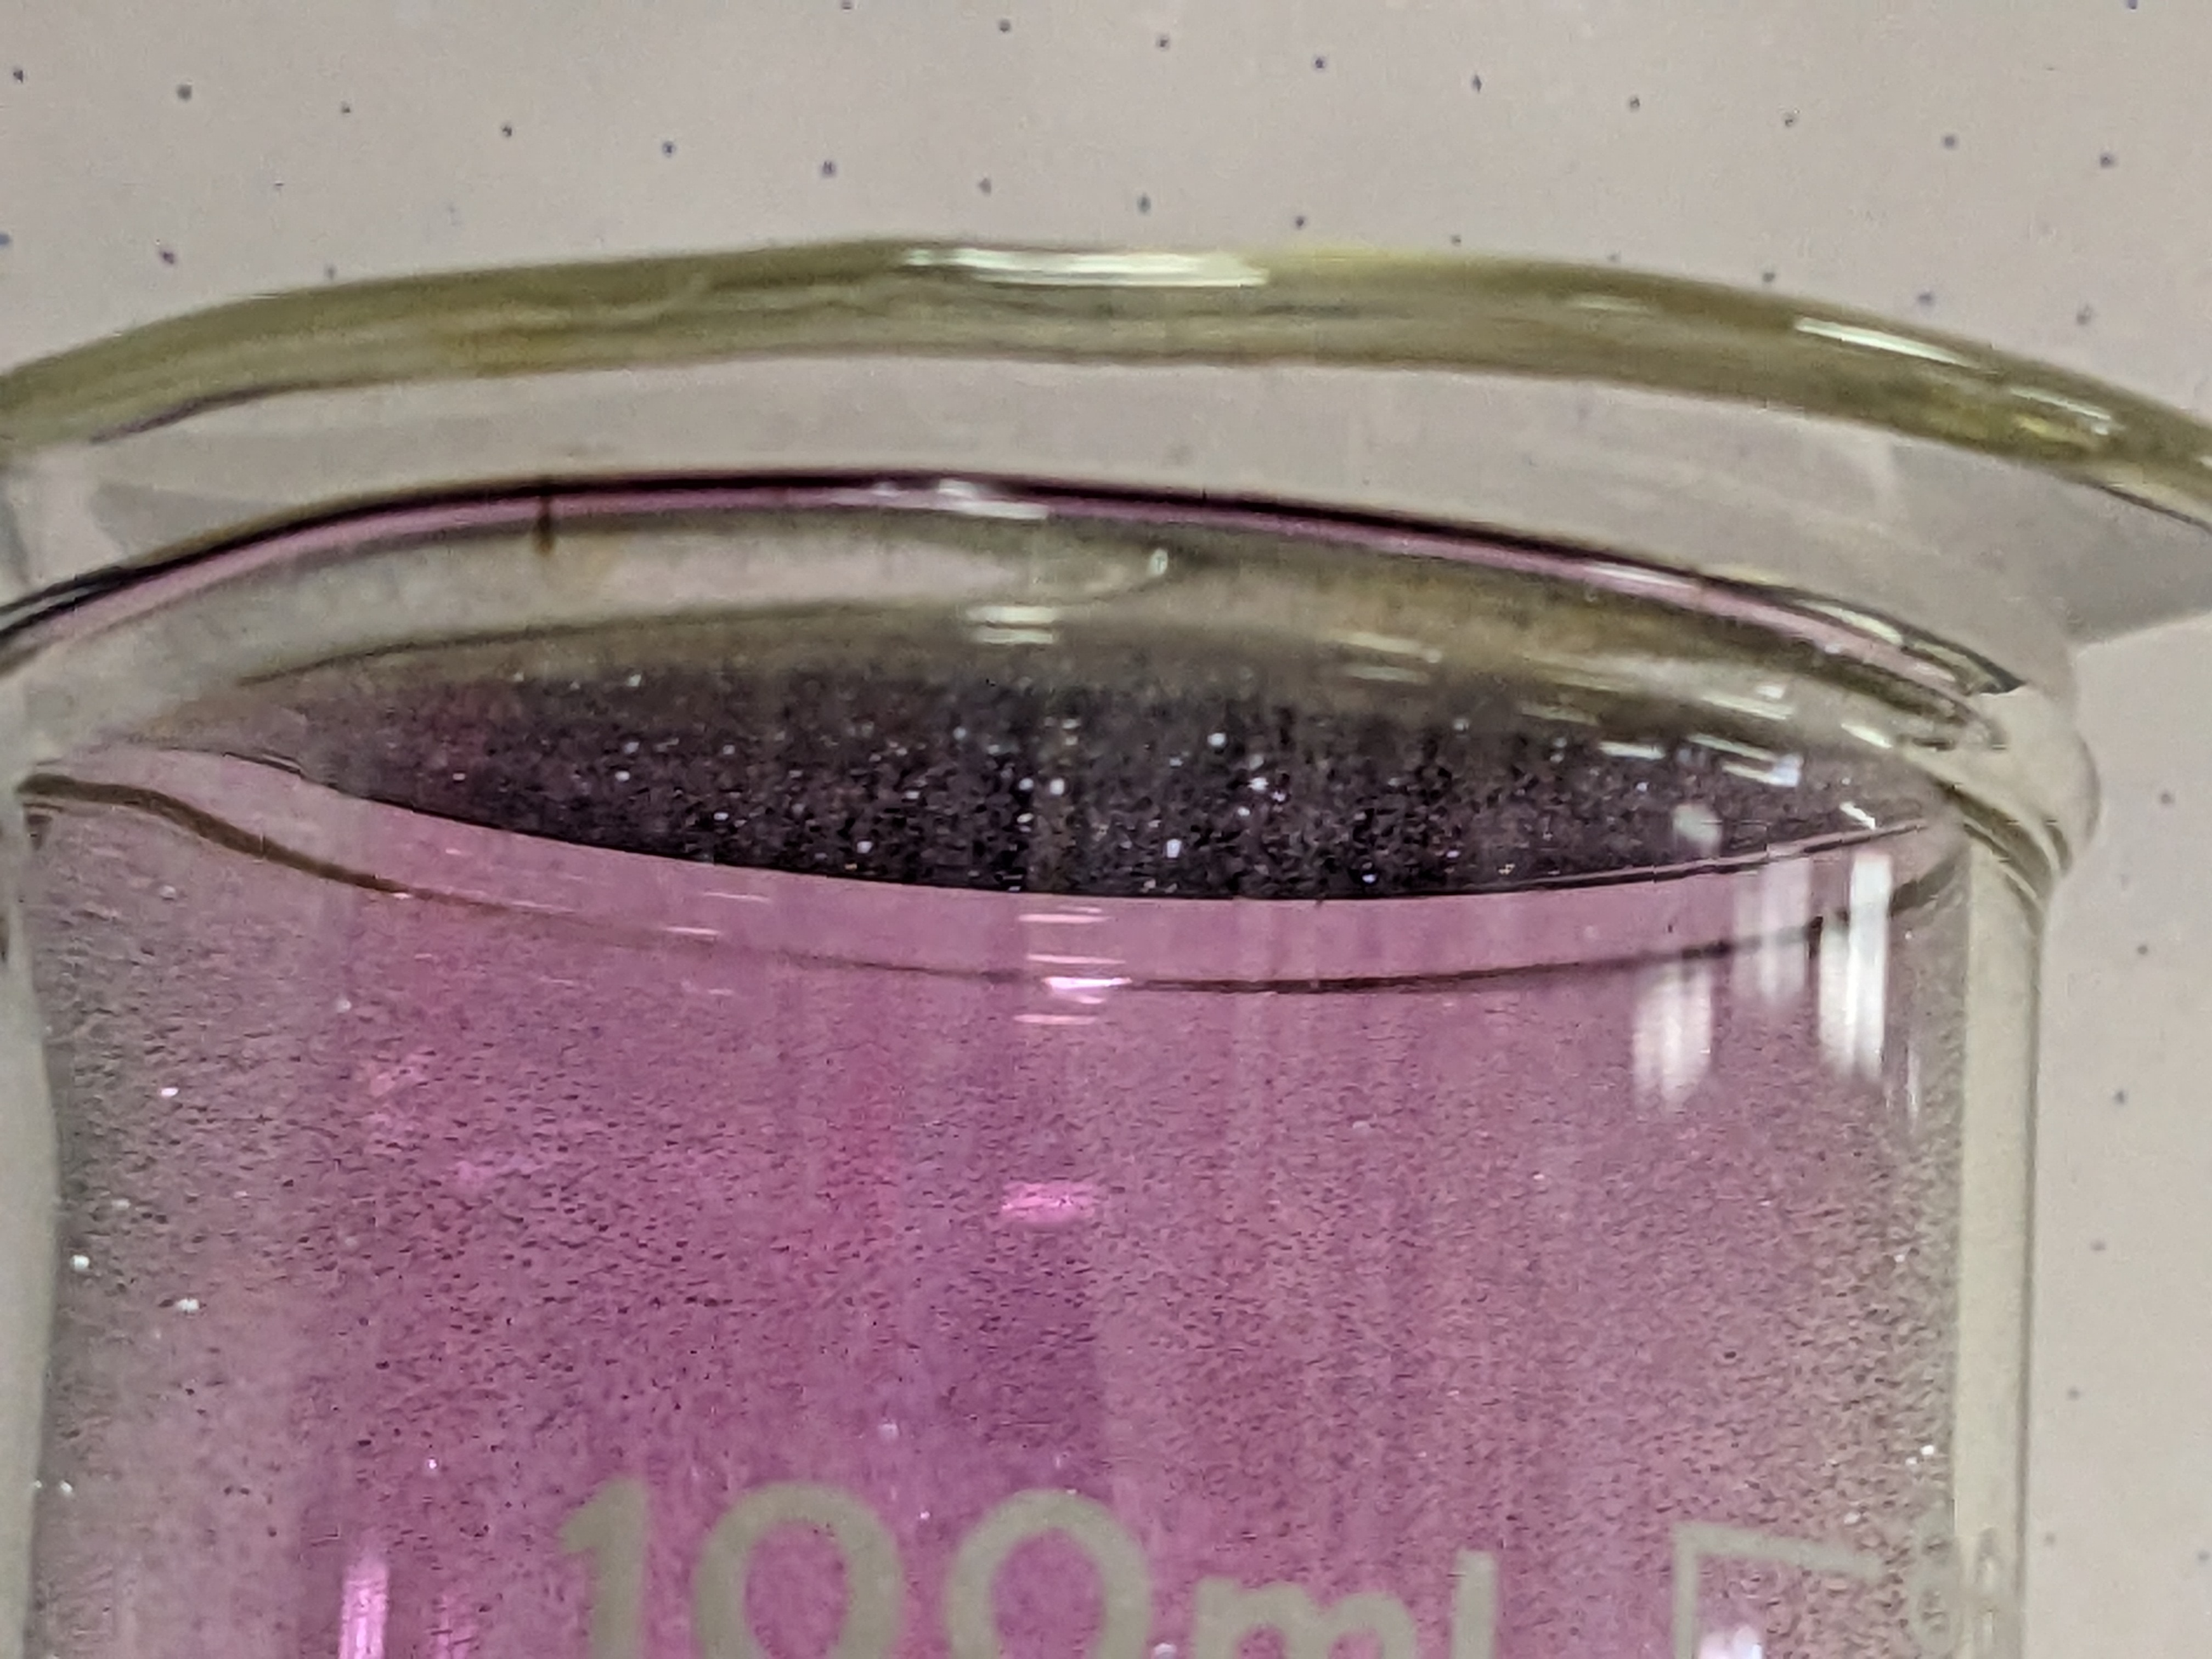
\includegraphics[height=3cm]{iodine_crystals.png} 
    \caption{Sublimation and deposition of \textbf{X}}
    \label{fig:heated_x}
\end{figure}

We found purple fumes coming off \textbf{X} and discoloration of the 'water' fascinating as it likely pointed to \textbf{X} being iodine. To further inspect \textbf{X} we wanted to see what would happen if we heated it up. We expected lots of purple vapor if \textbf{X} was indeed iodine. We took a few pieces of \textbf{X} and put them in a 100\unit{\milli\liter} beaker. We covered the beaker with a watch glass with some water on it and put it on the hot plate. As the beaker heated up, we observed more and more purple gas started to sublime from the solid \textbf{X}. At the top of the beaker, some of the gas deposited and formed spike-like crystals (Fig. \ref{fig:heated_x}).
% dont you not need to footnote after the 1st reference (on the 1st page)
% true

\bigskip
One really simple test for \textbf{M} was to test its magnetic properties. Holding a magnet next to a piece of \textbf{M} lead to no visible movement.

\begin{figure}[h]
    \centering
    \includegraphics[height=4cm]{activity_series.png} 
    \caption{Testing the reactivity of \textbf{M}}
    \label{fig:act_series}
\end{figure}

%will add molarity one i find them out
We performed a reactivity test on \textbf{M} exactly like how we did in our activity series lab. We used ten different metallic salt solutions: silver nitrate, aluminium nitrate, calcium nitrate, copper nitrate, iron nitrate, dilute hydrochloric acid, potassium nitrate, magnesium nitrate, stannous chloride in dilute hydrochloric acid, and zinc nitrate. Each of these solutions was contained in a dropper bottle. We took out ten pieces of \textbf{M} and lay them out on a laminated sheet. Over each piece, we added two to three drops of the respective solution. We then observed if a reaction took place (Fig. \ref{fig:act_series}). We observed that silver nitrate reacted with \textbf{M} and turned black, copper nitrate reacted with \textbf{M} and also turned black, iron nitrate reacted with \textbf{M} and created a yellow crust, hydrochloric acid reacted with \textbf{M} and bubbles formed, and stannous chloride in hydrochloric acid reacted with \textbf{M} and bubbles formed. Everything else gave no reaction.

%

\section{Gathered Data}

\section{Calculations}
%stoichiometry for MX first trial
% theoretical yield
% lets worry abt error prop later
\begin{gather*}
    \ce{Zn + I2 -> ZnI2} \\[2ex]
    \SI{0.512}{\gram\of{Zn}}\times\frac{\SI{1}{\mol\of{Zn}}}{\SI{65.380}{\gram\of{Zn}}}\times\frac{\SI{1}{\mol\of{Zn}}}{\SI{1}{\mol\of{\ce{ZnI2}}}}\times\frac{\SI{319.18}{\gram\of{\ce{ZnI2}}}}{\SI{1}{\mol\of{\ce{ZnI2}}}}=\SI{2.50}{\gram\of{\ce{ZnI2}}} \\[2ex]
    \SI{0.494}{\gram\of{I}}\times\frac{\SI{1}{\mol\of{I}}}{\SI{126.90}{\gram\of{I}}}\times\frac{\SI{1}{\mol\of{\ce{ZnI2}}}}{\SI{2}{\mol\of{I}}}\times\frac{\SI{319.18}{\gram\of{\ce{ZnI2}}}}{\SI{1}{\mol\of{\ce{ZnI2}}}}=\boxed{\SI{0.621}{\gram\of{\ce{ZnI2}}}} \\[2ex]
    \frac{\SI{0.523}{\gram}\mathrm{\ actual\ yield}}{\SI{0.621}{\gram}\mathrm{\ theoretical\ yield}}=\boxed{84.7\unit{\percent}\mathrm{\ yield}}
\end{gather*}

\begin{gather*}
    \SI{0.494}{\gram\of{I}}\times\frac{\SI{1}{\mol\of{I}}}{\SI{126.90}{\gram\of{I}}}\times\frac{\SI{1}{\mol\of{Zn}}}{\SI{2}{\mol\of{I}}}\times\frac{\SI{65.380}{\gram\of{Zn}}}{\SI{1}{\mol\of{Zn}}}=\SI{0.127}{\gram\of{Zn}}\mathrm{\ consumed} \\[2ex]
    \SI{0.512}{\gram\of{Zn}}-\SI{0.127}{\gram\of{Zn}}\mathrm{\ consumed}=\SI{0.385}{\gram\of{Zn}}\mathrm{\ remaining}
\end{gather*}
%%%
%\begin{gather*}
%    \rho_\textbf{M} = \frac {m_\textbf{M}}{V_\textbf{M}}
%\end{gather*}
%%%

\begin{gather*}
    m_\textbf{M} = \boxed{0.444 \pm 0.001  \,\si{\gram}} \\[2ex]
    V_\textbf{M} = \Delta V = V_{\mathrm{final}} - V_{\mathrm{init}} \\[2ex]
    V_\textbf{M} = 6.30 \,\si{\milli\liter} - 6.24  \,\si{\milli\liter} = 0.06 \,\si{\milli\liter}\\[2ex]
    \delta V_\textbf{M} = \sqrt{\delta V_{\mathrm{final}}^2+\delta V_{\mathrm{init}}^2} = \sqrt{(\SI{0.1}{\milli\liter})^2+(\SI{0.1}{\milli\liter})^2} = \sqrt{\SI{0.02}{\milli\liter}^2} = \SI{0.14}{\milli\liter} \\[2ex]
    V_\textbf{M} = \boxed{0.06 \pm 0.14 \,\si{\milli\liter}} \\[2ex]
    \rho_\textbf{M} = \frac {m_\textbf{M}}{V_\textbf{M}} = \frac{\SI{0.444}{\gram}}{\SI{0.06}{\milli\liter}} = 7.4 \,\si{\frac{\gram}{{\centi\meter}^3}} \\[2ex] 
    %\frac{\delta \rho_\textbf{M}}{\rho_\textbf{M}} = \sqrt{\left(\frac{\delta m_\textbf{M}}{m_\textbf{M}} \right)^2 + \left(\frac{\delta V_\textbf{M}}{V_\textbf{M}} \right)^2} = \sqrt{\left(\frac{\SI{0.001}{\gram}}{\SI{0.444}{\gram}} \right)^2 + \left(\frac{\SI{0.14}{\milli\liter}}{\SI{0.06}{\milli\liter}} \right)^2} = \sqrt{\left(\frac{\delta m_\textbf{M}}{m_\textbf{M}} \right)^2 + \left(\frac{\delta V_\textbf{M}}{V_\textbf{M}} \right)^2}\\[2ex]
    %help with sig figs :sob:
\end{gather*}

% trial 2
\large{Trial 2}
\begin{gather*}
    \ce{Zn + I2 -> ZnI2} \\[2ex]
    \SI{0.219}{\gram\of{Zn}}\times\frac{\SI{1}{\mol\of{Zn}}}{\SI{65.380}{\gram\of{Zn}}}\times\frac{\SI{1}{\mol\of{Zn}}}{\SI{1}{\mol\of{\ce{ZnI2}}}}\times\frac{\SI{319.18}{\gram\of{\ce{ZnI2}}}}{\SI{1}{\mol\of{\ce{ZnI2}}}}=\SI{1.07}{\gram\of{\ce{ZnI2}}} \\[2ex]
    \SI{0.194}{\gram\of{I}}\times\frac{\SI{1}{\mol\of{I}}}{\SI{126.90}{\gram\of{I}}}\times\frac{\SI{1}{\mol\of{\ce{ZnI2}}}}{\SI{2}{\mol\of{I}}}\times\frac{\SI{319.18}{\gram\of{\ce{ZnI2}}}}{\SI{1}{\mol\of{\ce{ZnI2}}}}=\boxed{\SI{0.244}{\gram\of{\ce{ZnI2}}}} \\[2ex]
    \frac{\SI{0.209}{\gram}\mathrm{\ actual\ yield}}{\SI{0.244}{\gram}\mathrm{\ theoretical\ yield}}=\boxed{85.7\unit{\percent}\mathrm{\ yield}} \\[2ex]
    \SI{0.194}{\gram\of{I}}\times\frac{\SI{1}{\mol\of{I}}}{\SI{126.90}{\gram\of{I}}}\times\frac{\SI{1}{\mol\of{Zn}}}{\SI{2}{\mol\of{I}}}\times\frac{\SI{65.380}{\gram\of{Zn}}}{\SI{1}{\mol\of{Zn}}}=\SI{0.0500}{\gram\of{Zn}}\text{ consumed} \\[2ex]
    \SI{0.219}{\gram\of{Zn}}-\SI{0.0500}{\gram\of{Zn}}\text{ consumed}=\SI{0.169}{\gram\of{Zn}}\text{ remaining} \\[2ex]
    \frac{\Delta m}{m}=\frac{\SI{0.169}{\gram\of{Zn}}\text{ theoretical remaining}-\SI{0.168}{\gram\of{Zn}}\text{ measured remaining}}{\SI{0.169}{\gram\of{Zn}}\text{ theoretical remaining}}=\SI{0.6}{\percent}\text{ error}
\end{gather*}

\section{Analysis}

The evidence we have to support the claim that the identity of the unknown element M is zinc falls into three categories. The first of these categories are the general properties of M. We first observed that M was made of small pieces cut from a larger sheet of metal, and was untarnished, but not extremely shiny. We next observed that M was very conductive, with only \SI{0.612}{\ohm} of resistance across 3mm of its surface. Furthermore, we found that M was malleable, and was able to be formed slightly with our hands. M's appearance and properties of conductivity and malleability are all properties of metals. Since M has many of the properties intrinsic to metals, we conclude that M is a metallic element. 

The next piece of evidence that supports M's identity as zinc is its reactivity. By performing reactivity tests against other metals, we can determine M's reactivity relative to other known metals. We found that M was more reactive than silver, copper, iron, tin, and hydrogen. We found that it was unable to replace calcium, potassium, magnesium, aluminium, and zinc. This exactly matches where zinc lies on the activity series, above the elements that M was able to replace, and below those it could not. However, since we did not have a chromium nitrate solution, and chromium is another metal that would match our reactivity results, we are unable to confidently verify M's identity as zinc from the activity series alone. However, in our next test, we are able to eliminate chromium as possibility for M's identity.

The final piece of evidence that allows us to confidently state M's identity as zinc is a flame color test. By reacting M and X, we were able to produce an ionic compound with M as the cation. \footnote{Verification of this fact is provided in the analysis of X's identity}When a metal ion is heated in a flame test, its electrons rise and fall between orbitial energy levels and emit a characteristic spectrum of light. Since all elements have unique energy levels, they have unique emission spectra, meaning the emitted spectrum of light from a flame test can be used to identify the element. Following our synthesis of MX with M as a cation, we dissolved the powder in methanol, and ignited it. We observed a pale, light blue flame. As a control, we also ignited pure methanol and observed a colorless flame. The two possibilities for M's identity that we obtained from our reactivity testing, zinc and chromium, have pale blue and silver white flames respectively. \footnote{insert citation} Since the observed flame color of our unknown is very different from that of chromium's, we are able to eliminate chromium as a possibility for our unknown's identity. However, there are a group of elements that have a flame color similar to our unknown. These include: arsenic, lead, tin, and zinc. However, using our initial observations as well as the reactivity of M, we are able to eliminate all of these possibilities, save for zinc. Therefore, by using evidence from all of our testing on M, we are able to confidently state the identity of M as zinc.


\bibliographystyle{alpha}
\bibliography{sample}

% 
% \setcrambond{2pt}{}{}
% \chemfig{
%   HO-[2,.5,2]?<[7,.7](-[2,.5]OH)-[,,,,line width=2.4pt](-[6,.5]OH)>[1,.7]
%     (-[:-65,.7]O-[:65,.7]?[b](-[2,.7]CH_2OH)<[:-60,.707](-[6,.5]OH)
%       -[,,,,line width=2.4pt](-[2,.5,,2]HO)>[:60,.707](-[6,.5]CH_2OH)-[:162,.9]O?[b])
%   -[3,.7]O-[4]?(-[2,.3]-[3,.5]HO)}
% 
% \setatomsep{2em}
% \chemfig{
%   H_3C-[:72]{\color{blue}N}
%     *5(-
%       *6(-(={\color{red}O})-{\color{blue}N}(-CH_3)-(={\color{red}O})-{\color{blue}N}(-CH_3)-=)
%     --{\color{blue}N}=-)}
% 
\end{document}
